%!TEX root = main.tex

\section{Core Concepts and Mechanisms}
\label{sec:core}

\subsection{System Model}

Each processing pipeline in Flink is first defined into a logical directed graph $G = (\mathcal{T}, \mathcal{E})$ where $\mathcal{T}$ is a set of vertices representing compute tasks and $\mathcal{E}$ is a set of edges representing data subscriptions between tasks in $\mathcal{T}$ (\autoref{fig:graphs}(a)). Data subscriptions can apply arbitrarily between tasks in $\mathcal{T}$, addressing the dependencies prescribed directly or indirectly via the programming model (e.g., forward, shuffle and hash partitioning). A task $t \in \mathcal{T}$ can encapsulate the logic of a single operation (e.g., \texttt{map}, \texttt{filter}, \texttt{fold}, \texttt{window}). However, standard logical dataflow optimisations  such as fusion \cite{hirzel2014catalog,chambers2010flumejava} are also applied in an intermediate step allowing multiple operators to share the same task in $\mathcal{T}$ (\autoref{fig:graphs}(b)). Each logical graph is directly mapped to a physical, distributed graph $G^*$ upon deployment or rescaling (\autoref{fig:graphs}(c)). In the rest of this section we are going to introduce the concept of managed state in Apache Flink, followed by physical state partitioning and a description of how state and data are being allocated to tasks.

\begin{figure}[t]
\centering
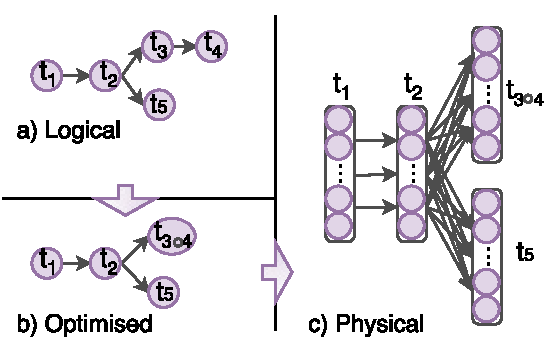
\includegraphics[width=\textwidth / 2]{figures/graphs.pdf}
\vspace*{-5mm}
\caption{Dataflow Graph Representation Examples.} 
\label{fig:graphs}
\vspace{-4mm}
\end{figure}

\subsubsection{Managed State}
\label{sec:managedstate}
Each stream operation in Flink can declare its own state and update it continuously in order to keep a summary of the data seen so far. State is a main building block of a pipeline as it encapsulates, at any time, the full status of the computation. There are conceptually two scopes upon which managed state operates. For purely data-parallel stream operations such as for example a per-key average, the computation, its state and associated streams can be logically scoped and operate independently for each key. This is similar to how a relational \texttt{GROUP\_BY} projects rows of the same key to the same set to compute grouped aggregates. We refer to this state as \texttt{Keyed-State}.
For local, per-task computation such as for example a partial machine learning training model, state can be declared in the level of a parallel, physical dataflow task, known as \texttt{Operator-State}. Both \texttt{Keyed-State} and \texttt{Operator-State} are transparently partitioned and managed by the runtime of the system. More importantly, the system can guarantee that update operations on managed state will be reflected exactly-once with respect to the input streams. In \autoref{sec:implementation} we explain in detail how the file system facilitates efficient external state persistence of different state types despite the local view exposed to the programmer. Below, we briefly explain how managed state can be declared and the basic intuition for each of the state types. 

%\stephan{I think we should write "he system can guarantee that update operations on managed  state  will be REFLECTED exactly-once with respect to the input streams. That more accurately captures the approach of rollback plus replay.}

\para{\texttt{Keyed-State}}: Any data-parallel stream computation can be mapped to a user-defined key space and as a result any associated state will also be scoped together with the computation. Typically, data-stream records arrive to the system with some domain-specific key such as a user-session identifier, a device address or a geographical location. In the most general case, Flink allows for a user to map any record from its schema domain $\mathcal{S}$ to a given key space $\mathcal{K}$ via the $\texttt{keyby}: \mathcal{S} \rightarrow \mathcal{K}$ operation supported by the \texttt{DataStream} abstract type. Under key scope, state can be allocated dynamically within a user-defined function by using special collections that the model exposes through the API and vary depending on the nature of the state. For append-only state per key (e.g. for storing a pattern sequence or a window) there is a \texttt{ListState} collection supporting an \texttt{add} operation. If  the state is otherwise a value that mutates during the application logic, there is a \texttt{ValueState} type supporting an \texttt{update} operation. Other basic state types such as \texttt{ReduceState} further allow for one or two-step, on-the-fly, distributive function aggregations on managed state. Finally, the \texttt{MapState} state type can support \texttt{put} and \texttt{get} key-value operations and is preferred over having a custom map declared as a \texttt{ValueState} as it avoids a full map deserialization to perform single key lookups.

\para{\texttt{Operator-State}}: Another scope upon which state and computation can be declared is within the granularity of each parallel instance of a task (task-parallel). \texttt{Operator-State} is used when part of a computation is only relevant to each physical stream partition, or simply when state cannot be scoped by a key. A Kafka ingesting source operator instance for example that has to keep offsets to respective partitions in Kafka \cite{kreps2011kafka} is using this scope. \texttt{Operator-State} adheres to a \emph{redistribution pattern} that allows breaking state into finer-grained units, when possible, allowing the system to redistribute state when changing the parallelism of the operator (scale in/out).
%In cases where \texttt{Operator-State} state can be further divided into finer-grained units (e.g., in Kafka-ingesting data sources when each task instance has to keep track of multiple partitions in Kafka)


%the \texttt{ListState} type can be used to declare further state units. Both \texttt{Keyed-State} and \texttt{Operator-State} scopes can be used in combination within a single user-defined operator on Flink, allowing for multiple granularities to handle state and processing-logic.

%\stephan{I think a reference to ListState it hard to get for an unfamiliar reader. How about writing something like this: "Operator-State typically declares a "redistribution pattern" that described how to break the state into finer-grained units and how to redistribute state when changing the parallelism of the operator (scale in/out)."}

%such as the source instances of a pipeline that correspond to Kafka consumers that map an active offset per partition
%Operator-state types are similar to Keyed-State (i.e., \texttt{ListState}, \texttt{ValueState}), whereas
%, both scopes 


%\stefan{The last sentence is partially incorrect. Right now, there is only list state for operator state, but it is also semantically different. It resembles more a value state and the only purpose of providing it in a list is breaking it down to repartitionable units for rescaling. Before rescaling was introduced, this state was just one huge black box, and Flink could never reason about how to redistribute this. Now, the user can divide the state into multiple black boxes. While they are still opaque for Flink, the system is now free to redistribute them.}

\begin{figure*}[t]
\centering
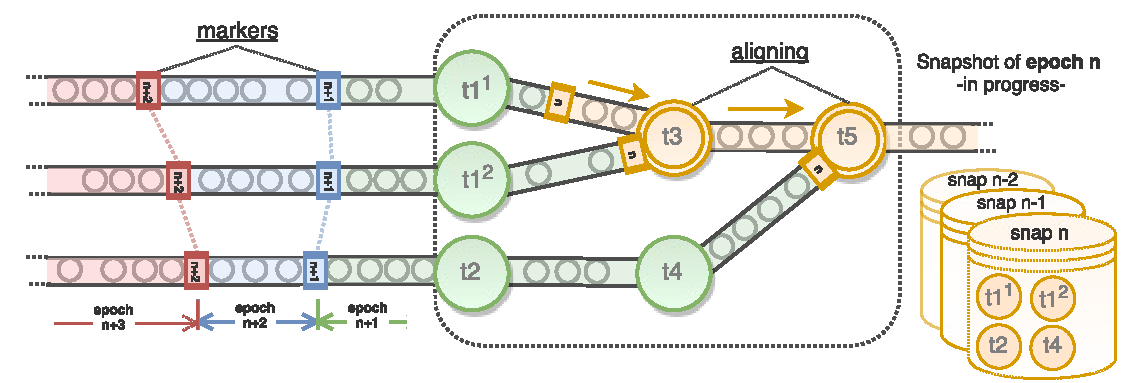
\includegraphics[width=\textwidth]{figures/snapshots-overview.pdf}
\vspace*{-10mm}
\caption{An Example of the Pipelined Snapshotting Protocol.} 
\label{fig:snapshots-overview}
\vspace{-4mm}
\end{figure*}


\subsubsection{State Partitioning and Allocation}

\para{Physical Representation}: The mapping of a logical graph $G$ to $G^* = \{\mathcal{T^*}, \mathcal{E^*}\}$, the physical, distributed execution graph (\autoref{fig:graphs}(c)) occurs when a pipeline is deployed, on its initial run or upon reconfiguration (e.g., for scale-out). During that stage each logical task $t \in \mathcal{T}$ is mapped to a number of physical tasks $t^1, t^2, \ldots, t^\pi \in \mathcal{T^*}$, each of which gets deployed to available containers throughout a cluster (e.g., using YARN \cite{vavilapalli2013apache} or Mesos \cite{hindman2011mesos}) up to the decided degree of parallelism $\pi \in \mathbb{N^+}$. 

\para{Key-Groups}: For tasks that have declared managed keyed state, it is important to consistently allocate data stream partitions or re-allocate in the case of reconfiguration. For flexibility, Flink decouples key-space partitioning and state allocation similarly to Dynamo\cite{decandia2007dynamo}. Consider a user-defined key space $\mathcal{K}$. The runtime maps keys to an intermediate circular hash space of ``key-groups'' : $\mathcal{K}^* \subset \mathbb{N^+}$ given a maximum parallelism $\pi\text{-max}$ and a hash function $h$ as such:

\noindent $\mathcal{K}^* = \{ h(k)\text{ \texttt{mod} }\pi\text{-max}\text{ }|\text{ }k \in \mathcal{K}, \pi\text{-max} \in \mathbb{N^+}, h: \mathcal{K} \rightarrow \mathbb{N^+} \}$

\noindent This mapping ensures that a single parallel physical task will handle all states within each assigned group, making a key-group the atomic unit for re-allocation. The intuition behind key-groups lies in the trade off between reconfiguration time (I/O during state scans) and metadata needed to re-allocate state (included within snapshots). On one extreme each parallel task could scan the whole state (often remotely) to retrieve the values of all keys assigned to it. This yields significant amounts of unnecessary I/O. 
%\stephan{("sequential" does not really add anything here. It is also not really guaranteed that this is always sequential, as the blob storage for the checkpoints can be a whatever. I would drop that term.)}  
On the opposite extreme, snapshots could contain references to every single key-value and each task could selectively access its assigned keyed states. However, this approach increases indexing costs (proportional to num. of keys) and communication overhead for multiple remote state reads, thus, not benefiting by coarse-grained state reads. Key-groups offer a substantial compromise: reads are only limited to data that is required and key-groups are typically large enough for coarse grained sequential reading (if $\pi\text{-max}$ is set appropriately low). In the uncommon case where $|\mathcal{K}| < \pi\text{-max}$ it is possible that some task instances simply receive no state.

%\stephan{This reads very "local disk" centric, where one optimizes for "sequential vs. random I/O". Is that the correct general terminology when talking about accessing data (remotely)? We could also use the terms "coarse grained" state access (reading/fetching a lot of unnecessary data) versus "many fine grained accesses" where the per-request overhead (remote request plus seek) makes it extremely expensive.}

\para{State Re-Allocation}: To re-assign state, we employ an equal-sized  key-group range allocation. For $\pi$ parallel instances, each instance $t^i \in \mathcal{T^*}, 0\leq i \leq \pi$ receives a range of key-groups from $\lceil i \cdot \frac{\pi\text{-max}}{\pi} \rceil$ to $\lfloor (i+1) \cdot \frac{\pi\text{-max}}{\pi} \rfloor$. Seeks are costly, especially in distributed file systems. Nevertheless, by assigning contiguous key-groups we eliminate unnecessary seeks and read congestion, yielding low latency upon re-allocation. 
\texttt{Operator-State} entries, which cannot be scoped by a key, are persisted sequentially (combining potential finer-grained atomic states defined across tasks), per operator, within snapshots and re-assigned based on their \emph{redistribution pattern}, e.g., in round-robin or by broadcasting the union of all state entries to all operator instances.
%Stephan: I think that is enough on the conceptual level - no need to go into more details here (it becomes very implementation specific otherwise).

%\stefan{You could use the black-box explanation that I mentioned in earlier comments. Operator-state is simply reassigned in round-robin, aiming to balance the number of assigned states among all tasks as much as possible. Additionally, we also have features called global and broadcast state. It is fully implemented, but currently not exposed in public API. This feature is based on replicating operator state from one task to all tasks upon restart, where replication means that all receiver read this from the same source, they just get a handle. In global state, we do a one-to-all replication (initially only one task has this task, upon restart it is replicated to all tasks), in broadcast state, we do all-to-all. }

\subsection{Pipelined Consistent Snapshots}
\label{sec:snapshots}

Flink's snapshotting protocol provides a uniform way to capture the complete state of a pipeline and roll it back whenever that is required. We will first explain its intuition followed by a more formal definition of the assumptions and description of the protocol for directed acyclic and cyclic graphs respectively.


\subsubsection{Approach Intuition}

A continuous stream execution is conceptually divided into logical periods that ``cut'' a distributed data stream into consecutive finite sets of records (\autoref{fig:snapshots-overview}), which we call \emph{epochs}. An \emph{epoch} can be triggered on-the-fly, periodically by the system or on-demand by the user and is decoupled from any application logic (e.g., windowing constrains). A snapshot of the computation at \emph{epoch} $n$ refers to a copy of the internal state of each task $t \in \mathcal{T^*}$ after the system fully ingests every input record from the beginning of the computation (\emph{epoch} 0) up to and including \emph{epoch} $n$. In case of a failure during or before a snapshot of \emph{epoch} $n$ is acquired we can simply revert the global state of the distributed dataflow graph to a previous \emph{epoch} (e.g., $n-1$). A discrete approach to snapshotting would be to let the system fully ingest \emph{epoch} $n$, log the internal state of each task $t \in \mathcal{T^*}$ and then proceed with \emph{epoch} $n+1$ (similarly to micro-batching \cite{zaharia2012discretized}). However, this approach raises latency and underutilization costs related to the coordination of a discrete execution which can be hard to amortize. Furthermore, other protocols either disrupt normal execution \cite{murray2013naiad,jacques2016consistent} or are incapable of supporting typical weakly connected graphs \cite{chandy1985distributed}.

Instead, Flink's snapshotting protocol pipelines progressively the partial acquisition of task states to eventually acquire a complete snapshot, respecting \emph{epochs}, while running concurrently alongside normal operation. Special markers are injected in each data stream partition at the dataflow sources, coordinated by the runtime and get disseminated throughout the dataflow graph as depicted in \autoref{fig:snapshots-overview}. Markers signal distributed tasks of new epochs and thus aid to establish the appropriate moment to snapshot each local state and proceed with further processing promptly. Tasks with multiple inputs execute an \emph{alignment} phase (e.g., tasks $t3$ and $t5$ in \autoref{fig:snapshots-overview}) upon which they prioritize exclusively inputs from pending \emph{epochs}. Alignment is decentralized and eliminates the need to fully consume an epoch or log records in transit before snapshotting. As we explain in more detail further, cyclic graphs require partial channel logging only limited to each dataflow cycle. The snapshotting protocol is coordinated centrally by the \emph{JobManager} and each invocation eventually completes or gets aborted (e.g., when a failure occurs). In either case the overall dataflow computation can always progress without interruptions and consecutive snapshots will eventually complete.

\subsubsection{Main Assumptions}

The protocol assumes a fail-recovery, deterministic process model \cite{elnozahy2002survey} where a partial process failure can be masked by redeployment and restoration of prior operational states. In detail, our protocol builds on the following assumptions:

%\begin{itemize}
\para{I}: Input data streams are durably logged and indexed externally allowing dataflow sources to re-consume their input, upon recovery, from a specific logical time (offset) by restoring their state. This functionality is typically provided by file systems and message queues such as Apache Kafka \cite{kreps2011kafka}
%\stephan{Minor comment: We don't actually need strict offset replay - we simply need to "mark" input such that we can replay from that "mark". This can also be obtained by deferring acknowledgement to the message queue, causing it to
%replay elements (as we do with RabbitMQ)}
%If that is not supported, similar logging functionality has to be implemented at the sources of the pipeline. 

\para{II}: Directional data channels between tasks are reliable, respect FIFO delivery and can be blocked or unblocked. When a channel is blocked, in-transit messages are internally buffered (and possibly spilled to disk) and can be delivered on that end once it unblocks.

\para{III}: 
Tasks can trigger a \texttt{block} or \texttt{unblock} operation on their input data channels and a \texttt{send} operation (records or control messages) on their output channels.
%\end{itemize}


\subsubsection{Directed Acyclic Graphs}

\begin{figure}[t]
\centering
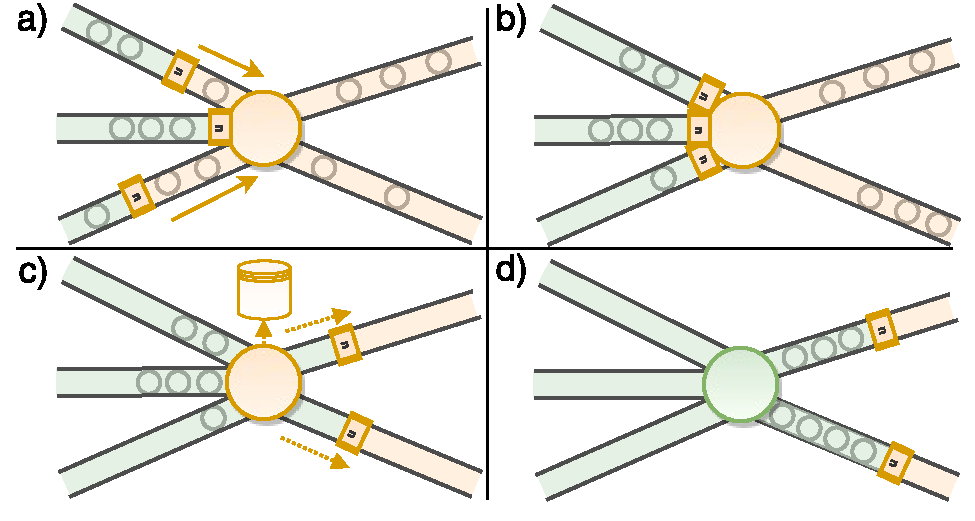
\includegraphics[width=\textwidth / 2]{figures/snapshots-highlights.pdf}
\caption{Alignment and Snapshotting Highlights.} 
\label{fig:snapshots-highlights}
\vspace{-2mm}
\end{figure}
\begin{figure}[t!]
\centering
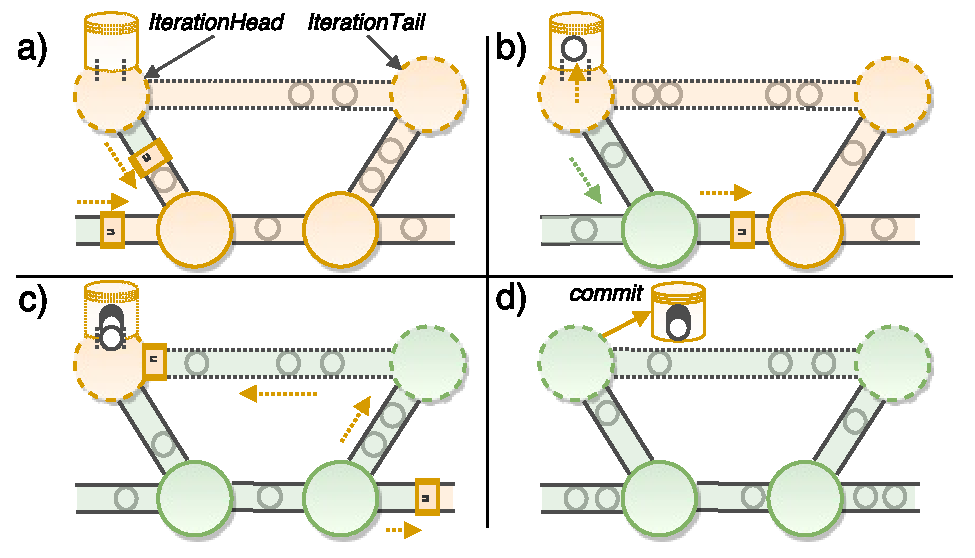
\includegraphics[width=\textwidth / 2]{figures/cycle-highlights.pdf}
\caption{Cycle Snapshotting Highlights.} 
\label{fig:cycle-highlights}
\vspace{-2mm}
\end{figure}


Let us consider only directed acyclic graphs (DAGs) for now. The protocol gets initiated at the source tasks of the dataflow by the \texttt{TaskManager}, however, for simplicity we assume here that the logic gets initiated upon receiving a special marker event in each and every task (sources would ``receive'' that first through a $Nil$ channel). \autoref{alg:snapdag} summarizes the snapshot alignment and pipelining protocol that executes when a marker is received. Mind that markers and records are handled sequentially by the same underlying thread that also invokes user-defined operators. 

\para{Alignment:} \autoref{fig:snapshots-highlights} vizualizes the steps prior to and during snapshotting in more detail. When a task receives a snapshot marker on one of its inputs, it blocks that channel since all computation associated with the current epoch has to finish before continuing further (\autoref{fig:snapshots-highlights}(a)). The blocking operation might result into spilling of in-transit records within that channel to disk, if allocated memory for network buffers reaches its limit. Once markers have been received in all inputs (\autoref{fig:snapshots-highlights}(b)) the task can further notify downstream tasks while also proceeding with snapshotting. Markers are first broadcasted forward and then local snapshotting is triggered, both of which can progress concurrently without sacrificing consistency (\autoref{fig:snapshots-highlights}(c)). Depending on the backend support, snapshots can be triggered and executed asynchronously by another thread, thus, minimizing their impact to the overall throughput. Once local snapshotting is initiated (\autoref{fig:snapshots-highlights}(d)) input channels are unblocked and regular operation continues to the next epoch. Overall, reliable FIFO data channels (Assumption II), combined with alignment guarantee that epoch-order is always respected. 

\para{Relaxing Consistency}: It is possible, if a pipeline allows for relaxed consistency requirements, to disable alignment (i.e., no input blocking). Essentially, this means that a snapshot on epoch $n$ will contain side-effects of input residing in epochs $\geq n$. Upon rollback records succeeding epochs $n$ are going to be ingested again, resulting into multiple state updates. This type of processing guarantees, also known as \emph{at-least-once processing}, can be enabled on Flink to trade-off consistency for practically zero latency impact if the application has no critical requirements.


\begin{algorithm}[h]
$inputs$ $\leftarrow$ configured\_inputs\;
$outputs$ $\leftarrow$ configured\_outputs\;
$blocked \leftarrow \emptyset$ \;
% $operator$ $\leftarrow$ dataflow\_operator\;

\Hdl{$\langle marker \rangle$ from $in \in inputs$}{
\If{$in \neq Nil$}{
 $blocked \leftarrow blocked \cup in$\;
 $in$.block()\;
}
\If{$blocked = inputs$}{
\ForEach{$out \in outputs$}{
$out$.send($\langle marker \rangle$)\;
}
triggerSnapshot()\;
\ForEach {$in \in inputs$}{
$in$.unblock()\;
}
$blocked \leftarrow \emptyset$ \;
}
}
\caption{Snapshot Alignment}
\label{alg:snapdag}
\end{algorithm}

\subsubsection{Dealing with Dataflow Cycles}

Dataflow graphs in Flink can also support cycles. Cycles are currently defined explicitly through Flink's programming API as asynchronous iterations, though bulk synchronous iterations (e.g., on stream windows) are also considered and can be supported in the future. Cyclic snapshotting is handled as a special case and implemented by system-specific, implicit tasks: an \texttt{IterationHead} and \texttt{IterationTail}. These tasks act as regular dataflow \emph{source} and \emph{sink} respectively, yet, they are collocated in the same physical instance to share an in-memory buffer and thus, implement loopback streams transparently.

The default stream alignment logic presented (\autoref{alg:snapdag}) would result into an incomplete distributed snapshot if applied on cyclic graphs. That is due to the fact that records belonging to prior epochs could still remain indefinitely in-transit within a cycle even after a snapshot has been taken over. Thus, it is crucial to persist these records in the snapshot in order to get a complete picture of the correct distributed execution \cite{chandy1985distributed,elnozahy2002survey}. Alternative approaches to this problem consider a ``flushing'' phase which enforces the inclusion of all the in-transit records to the internal state of each task \cite{jacques2016consistent}, however, we argue that this problem is only relevant to the state of a cycle. Thus, we execute a similar special logging protocol (\autoref{alg:snapcycle}) that runs solely within the \texttt{IterationHead} instances of each cycle.


As described in detail in \autoref{alg:snapcycle} and also visualized in \autoref{fig:cycle-highlights}, \texttt{IterationHead} tasks receive a special marker from the runtime signifying each epoch, same as the sources of the dataflow graph. At that instance, they disseminate markers further within a cycle and start logging in their own managed state all in-transit events that exist within a cycle in that respective partition (\autoref{fig:cycle-highlights}(a)). Once the marker of the snapshot is received back through their respective collocated \texttt{IterationTail} (\autoref{fig:cycle-highlights}(c)) they trigger a snapshot of that log containing a complete backup of all transmitted records in that epoch (\autoref{fig:cycle-highlights}(d)). Again, FIFO channels and alignment executed by the rest of the tasks within a cycle (\autoref{fig:cycle-highlights}(b)) ensures that no records from succeeding epochs will transit prior to the marker. This special logic also restricts channel logging to cycles and does not enforce anything other than task states to be included in the snapshot for the rest of the  graph.

%(unlike Chandy and Lamport's \cite{chandy1985distributed} algorithm or state-of-the-art protocols that focus on weakly connected dataflow graphs \cite{elnozahy2002survey,jacques2016consistent,murray2013naiad}).

\begin{algorithm}[t]
$outputs$ $\leftarrow$ configured\_outputs\;
$isLogging \leftarrow false$ \;
$log \leftarrow \emptyset$ \;

\Hdl{$\langle marker \rangle$}{
\eIf{$isLogging$}{
triggerSnapshot($log$) \;
$log \leftarrow \emptyset$ \;
$isLogging \leftarrow false$ \;
}{
$isLogging \leftarrow true$ \;
\ForEach{$out \in outputs$}{
$out$.send($\langle marker \rangle$)\;
}
}
}
\Hdl{$record$}{
\If{$isLogging$}{
 $log \leftarrow log \cup record$\;
}
\ForEach{$out \in outputs$}{
$out$.send($record$)\;
}
}
\caption{Snapshotting in Cycles}
\label{alg:snapcycle}
\end{algorithm}


\subsection{Usages and Consistent Rollback}

%\stephan{I would not even introduce the term "Savepoints" here, but simply stick with checkpoints/snapshots. More or less all checkpoints are externalized (at least in proper high availability setups). Mentioning that checkpoints can be explicitly archived for later rollback/reprocessing, etc makes sense. Other than that, I would simply mention that checkpoints define consistent points across parallel operators and thus are suitable points for reconfiguration. Reconfiguration conceptually happens via checkpoint/stop/modify/restore, but can also happen by attaching reconfiguration commands to barriers, which then reconfigure operators (replace code) at the point where the snapshot is taken. The later is not yet implemented (future work), but is worth mentioning in my opinion.}

Consistent snapshots, described previously in \autoref{sec:snapshots} form the basis for a variety of operations using the Apache Flink system. Periodic snapshots are automatically triggered by Flink's runtime as a form of per-job ``checkpoint'' for the purposes of consistent fail recovery whenever partial failures occur. However, the usages of snapshots go beyond fault tolerance needs. For a system that is widely deployed in a cloud infrastructure, having the ability to scale resources in or out and lease containers is nowadays a necessity. In principle, failover and re-scaling are two operations that share the same underlying need for consistent reconfiguration support \cite{castro2013integrating}. In this section we describe in more detail the operational benefits that distributed snapshots make feasible, as well as the rollback reconfiguration schemes that are currently supported.

\subsubsection{Snapshot Usages}
\label{sec:savepoints}

Flink's snapshots define consistent points across parallel operators and thus, are suitable points for reconfiguration. The metadata of a snapshot contains all necessary information required to retrieve the complete pipeline state from an associated durable storage backend such as references and indexes to operator state partitions (i.e., key-groups) and upstream logs (in case of cyclic graphs). Common causes of reconfiguration are: 1) application logic updates (e.g., software patches) of already running jobs by replacing operators accessing the same snapshotted state or adding new state entries instead and 2) application versioning, allowing forking running pipelines (an example depicted in \autoref{fig:savepoints}). In practice, reconfiguration follows a \texttt{checkpoint-stop-modify-restore} cycle, initiated externally by the user. However, it is also possible to be triggered topologically by attaching reconfiguration commands to snapshot markers which reconfigure operators (replace code) at the point where the snapshot is taken. 

\begin{figure}[t]
\centering
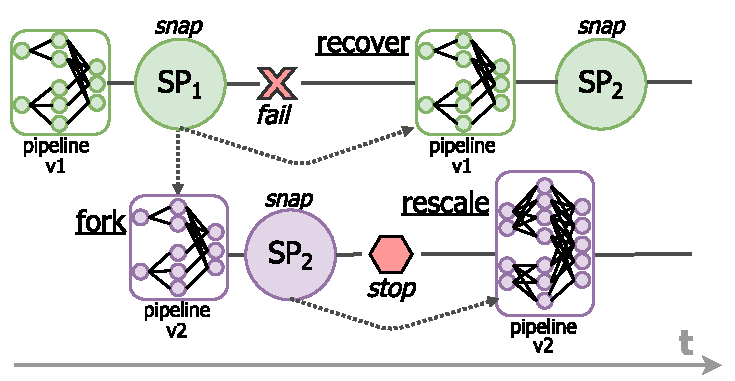
\includegraphics[width=\textwidth / 2]{figures/savepointsexamples.pdf}
\vspace{-6mm}
\caption{Snapshot usage examples.} 
\label{fig:savepoints}
\vspace{-4mm}
\end{figure}

%\paris{perhaps we could elaborate more here and add a motivating figure with snapshots and usages}
%\stefan{While savepoints and checkpoints are currently in the same format, we are planning to change this in the future. In particular, we are talking about costly features or properties, such as rescalability. We want to keep checkpoints as cheap as possible, at the cost of not supporting certain ops like rescaling from checkpoints. Savepoints, in turn, could be more costly but provide rescalability. Key-groups come with a certain cost, not only in meta data. Some backends may require some live partitioning before writing the snapshot. On top of that, key-groups can also mess with other natural groupings, such as namespaces that we find in windowing. For example, it would be nice to have locality for all keys in a window, so that we can quickly iterate over the window. However, we need to write data in key-group order, which forces us to split up the natural grouping of windows, into up to one partial window per key-group. Also in the context of incremental snapshotting, key-groups can easily become problematic. So checkpoints might support incremental snapshots, while savepoints might require full snapshots.}

\subsubsection{Consistent State Rollback}

Rollback recovery gets initiated upon a task failure or when there is a need to rescale. Typically, the latest snapshot is used to restart the application from the beginning of the latest committed epoch. Depending on the rollback cause, different recovery schemes are employed. For example. during a full restart or rescaling, all tasks are being redeployed, while after a failure only the tasks belonging to the affected connected component (of the execution graph) are reconfigured. In essence, known incremental recovery techniques from  micro-batch processing \cite{zaharia2012discretized} are orthogonal to this approach and can also be employed. A snapshot epoch acts as synchronization point, similarly to a micro-batch or an input-split. On recovery, new task instances are being scheduled and, upon initialization, retrieve their allocated shared of state. In the case of  \texttt{Iteration Head} recovery, all records logged during the snapshot are recovered and flushed to output channels prior to their regular record-forwarding logic. Eventually, all states within the pipeline are progressively retrieved and applied to reflect an exact, valid distributed execution at the restored epoch. 

%It is possible that a pipeline's dataflow graph consists of multiple weakly connected components. In case of a failure on a single of these connected components, rollback recovery can be applied only in the respective component, leaving other components' normal execution intact. This optimization yields a more fine-grained recovery scheme and does not violate consistency since there are no data dependencies across disconnected components. 

It is additionally required for all data sources to rollback input from the epoch where the snapshot occurred. Flink's data sources provide this functionality out-of-the-box by maintaining offsets to the latest record processed prior to an epoch from external logging systems. Upon recovery the aggregate state of those sources reflects the exact distributed ingestion progress made prior to the recovered epoch. This approach assumes that external logging systems, that sources communicate with, index and sequence data across partitions in a durable manner (e.g., Kafka, Kinesis, PubSub and Distributed File Systems). 

%\stephan{It is worth mentioning that techniques known from batch/mini-batch processing for incremental recovery are applicable here. The completed checkpoint is the point to restart from (similar to beginning of "input split" or beginning of "mini batch"). The only difference here is that downstream operators have to be rolled back as well, for exactly-once semantics (or not, for at-least-once semantics).}
%\paris{Maybe explain briefly how unreliable sources can work}

%Alternatively each data source instance has to maintain a durable write-ahead-log 
%of all uncommitted input and delay ingestion by an epoch to emulate the same assumptions through Flink's snapshotting mechanism.



